% TODO:  change space between items
\documentclass[12pt,a4paper]{article}
%\usepackage{fontspec}
\usepackage{float}
\usepackage{graphicx}
\usepackage{framed}
\usepackage[inline]{enumitem}
\usepackage{footnote}

\usepackage{caption}
\captionsetup{margin=10pt,font=small,labelfont=bf}
\usepackage{subcaption}

\usepackage[ linktocpage=true]{hyperref}
\hypersetup{
	colorlinks=true,
	breaklinks=true,
	pdfinfo={
		Title={Technical Analysis and Backtesting 
			From Scratch -- A Demonstration},
		Subject={Technical Analysis},
		Author={Kong Shuai},
		Recipients={}
	}
}

\usepackage[numbered]{bookmark}

\begin{document}
%\title{Technical Analysis and Backtesting\\ From Scratch
%	\\[2ex]--- A Demonstration}
	
\title{Technical Analysis and Backtesting\\ From Scratch
	\\[2ex]--- A Demonstration\footnote{
			The framework of this project is 
			written in Python -- a powerful programming language. 
			Most of the figures are produced with R, 
			and this document is written with \LaTeX{}.}
%		\footnote{The main reasons include:
%			\emph{a}) prices are not properly adjusted against 
%				splits and dividends;
%			\emph{b}) prices on Yahoo! 
%				are said not always to be accurate;
%			\emph{c}) it is not fully tested and
%			\emph{d}) the demo is not built on a credible theory.}
			}

	
\author{Kong Shuai\\
kongshuai89@gmail.com}
\date{February 15, 2013}
\maketitle

%\begin{center}
%\begin{minipage*}[c]{\textwidth}
%\fbox{\parbox{\textwidth}{
%	\begin{large}IMPORTANT\end{large}:
%	This is a demonstration aimed at showing the possibilities
%	with the help of IT skills\footnote{The framework of this project is 
%		written in Python -- a powerful programming language. 
%		Most of the figures are produced with R, 
%		and this document is written with \LaTeX.}. 
%	Conclusions should NOT be considered as applicable to the real 
%	circumstance\footnote{The main reasons include
%		\begin{enumerate*}[label=\emph{\alph*}), before=\unskip{: }, 
%					itemjoin={{; }}, itemjoin*={{, and }}]
%			\item prices are not properly adjusted against 
%				splits and dividends
%			\item prices on Yahoo! are said not always to be accurate
%			\item it is not fully tested
%			\item the demo is not built on a credible theory.
%		\end{enumerate*}}.
%	}}
%\end{minipage*}
%\end{center}

\begin{framed}
	\begin{large}IMPORTANT\end{large}:
	This is a demonstration aimed at showing the possibilities
	with the help of IT skills. 
	Conclusions should NOT be considered as applicable to the real 
	circumstance\footnotemark.
	\bigskip
	
	Please do NOT make me public on the web!
\end{framed}


\footnotetext{The main reasons include:
			\emph{a}) prices are not properly adjusted against 
				splits and dividends;
			\emph{b}) prices on Yahoo! 
				are said not always to be accurate;
			\emph{c}) it is not fully tested and
			\emph{d}) the demo is not built on a credible theory.
			}

\section{Overview}

\subsection{Birth}
When I was asked to helped a friend with an essay on 
APT (Arbitrage Pricing Theory) a year ago (2012),
the first problem was how to get enough stock prices without dirty work.
And when I worked it out through the API of Yahoo! Finance with 
Python\footnote{Python is a remarkably powerful dynamic programming language 
that is used in a wide variety of application domains. Details
can be found at the official website: http://www.Python.org/.},
I realized I can do something more than the essay, maybe something about 
technical analysis.

\subsection{Project Task}
\begin{itemize}[itemsep=0pt]
\item Build up a framework of technical analysis, with which user can:
	\begin{itemize}[nosep]
	\item Build up a user defined trading strategy.
	\item Test the strategy with various stocks (backtesting).
	\end{itemize}
\item With the basics built up, test whether the common parameters of classic 
technical analysis are still the best from a statistical perspective.
\end{itemize}

So, the implementation include the following main components:
\begin{itemize}[itemsep=0pt]
\item A local data source to store and provide historical price.
\item A framework to define and back-test strategies.
\item Data analysis.
\end{itemize}


\section{Local Data Source}
The local data source is used to store necessary stocks information, 
like the corresponding companies and the sectors they belong to, 
which may be used when considering difference among sectors.

\subsection{Storage}
As the data can be quite large and concentrated on a single table,
I set up a PostgreSql database to store it.

\subsection{Update}
Downloading and updating the historical prices are done 
with a Python script.
This script downloads prices from Yahoo automatically 
according to the symbols pre-stored in the database, 
and update the local data source when new price records are found.


\section{Technical Analysis Framework}
Again I choose Python as the programming language. Considering that 
there may be quite a lot of calculations, 
I built it up on the widely used packages, 
NumPy\footnote{NumPy is the fundamental package 
for scientific computing with Python.}~and 
matplotlib\footnote{matplotlib is a Python 2D plotting library 
which produces publication quality figures in a variety of hardcopy 
formats and interactive environments across platforms.}, 
when Python are introduced into scientific fields.

%\subsection{Prices and Stocks}
Price and stock are wrapped into class to contain necessary information
and useful method. Price is a component of stock, and strategies are 
supplied with stock objects.

%\subsection{Strategies}
Basic or standard strategies like MA are written and can be used as a 
component when building up a more complicated strategy like MACD.

User defined strategy can also be written here like the MACD. 
The good part is that 
users are fully benefit from the advantages that Python provide.

As the main purpose is to enable backtesting, and considering 
that most trading programs provide fine figures,
plotting is not a main aspect here,
but in order to provide a some kind of \emph{visual} result, I write a simple
example of MACD, which looks like the 
Figure~\ref{fig:macd-plot} on p.~\pageref{fig:macd-plot}.


\begin{figure}[H]
\centering
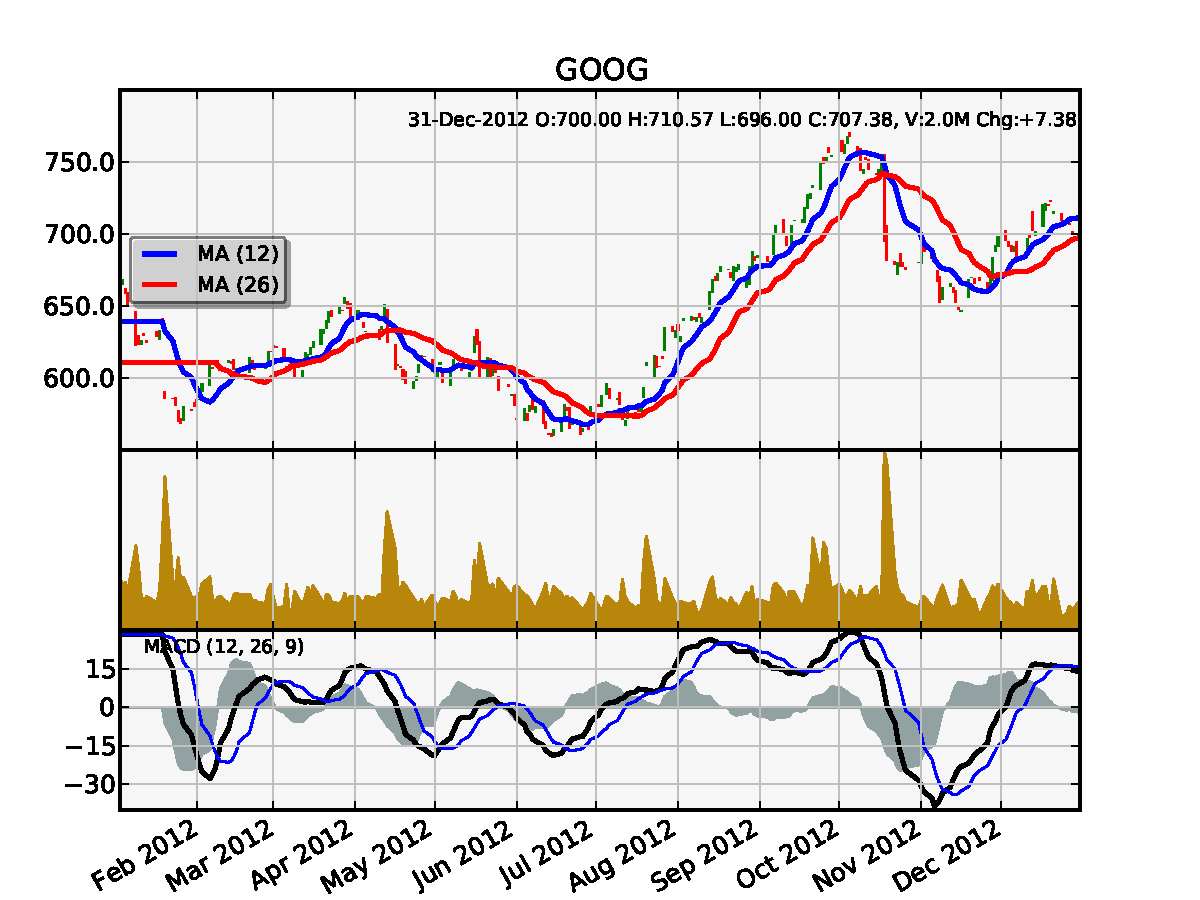
\includegraphics[width=\textwidth]{image/macd-plot.pdf}
\caption{A MACD Figure by Python with Matplotlib\label{fig:macd-plot}}
\end{figure}

\section{Data Analysis}
With NumPy and SciPy\footnote{SciPy is open-source software for 
mathematics, science, and engineering. 
It is also the name of a very popular conference 
on scientific programming with Python.}~package, 
it is also possible to do the analysis inside 
the framework built up before. But because the raw data 
is usually very regular, so doing this with a 
specialized program like R\footnote{
R is a language and environment for statistical computing and graphics. 
It is a GNU project which is similar to the S language and environment 
which was developed at Bell Laboratories 
by John Chambers and colleagues.}, could be a better idea.

\subsection{MACD Parameters[Demo]}
Here is a very simplified and not rigorous example. 
It should NOT be used in practice matters.

A general guess is that, as information spread much faster than before,
should the MACD arguments selected be \emph{smaller}?

There are mainly three meaningful signals generated by the MACD indicator
that traders recognize. As a simple demo, only one signal is considered
in the following steps -- when MACD line crosses the signal line, where 
\[\mathrm{MACD = MA_{fast} - MA_{slow}} \]
and
\[\mathrm{signal = EMA(MACD, 9)}\]

\subsubsection{Revenue Distribution}
With the help of the framework above, the revenue of a stock 
can be calculated easily like $\mathrm{MACD(n_{fast}, n_{slow}, n_{macd})}$.
I run this on 30 DJIA component stocks and get a list of about 95,000 
records, see Figure~\ref{fig:revenue} on p.~\pageref{fig:revenue}.


In this figure, dash line is the density of revenue, 
while the thick line is the density of 
normal distribution with the same mean and variance of revenue.

\begin{figure}[H]
\centering
\includegraphics[width=\textwidth]{image/revenue-hist.pdf}
\caption{Distribution of Revenue\label{fig:revenue}}
\end{figure}


\subsubsection{Revenue and Parameter}
In order to see the effect of parameter values, 
we can plot the revenue on each $\mathrm{n_{fast}}$ 
and $\mathrm{n_{slow}}$. R can do
this easily with its formula expression.

Figure~\ref{fig:revenue-by-par} on p.~\pageref{fig:revenue-by-par}
gives a general view. Figure~\ref{fig:revenue-by-par:nfast} shows the 
boxplot of revenue in respect of different $\mathrm{n_{fast}}$, and 
\ref{fig:revenue-by-par:nslow} of $\mathrm{n_{slow}}$. 
In this figure we can see than the 
classic (12, 26) is probably not the best.


%\begin{figure}[htbp]
%\centering
%\subfloat[][Revenue of Each $n_{fast}$\label{fig:revenue-by-par:nfast}]{
%
%\includegraphics[width=.4\textwidth, height=!]{image/revenue-nfast2.pdf}
%}
%
%\subfloat[][Revenue of Each $n_{slow}$\label{fig:revenue-by-par:nslow}]{
%\includegraphics[width=.5\textwidth, height=!]{image/revenue-nslow2.pdf}
%}
%\caption{Revenue Categorized by Parameter Value}
%\label{fig:revenue-by-par}
%\end{figure}

\begin{figure}[htbp]
\begin{subfigure}[b]{.5\textwidth}
\centering
\includegraphics[width=\textwidth, height=!]{image/revenue-nfast2.pdf}
\caption{Revenue of Each $\mathrm{n_{fast}}$}
\label{fig:revenue-by-par:nfast}
\end{subfigure}
\begin{subfigure}[b]{.5\textwidth}
\centering
\includegraphics[width=\textwidth, height=!]{image/revenue-nslow2.pdf}
\caption{Revenue of Each $\mathrm{n_{slow}}$}
\label{fig:revenue-by-par:nslow}
\end{subfigure}
\caption{Revenue Categorized by Parameter Value}
\label{fig:revenue-by-par}
\end{figure}


A numerical summary can be found in Table~\ref{tab:revenue-by-nfast}.
When let $\mathrm{n_{fast}}$ be 8, 9, 10, 11, the summary fields are 
all better than of 12.



% latex table generated in R 2.15.2 by xtable 1.7-0 package
% Tue Feb 12 20:20:19 2013
\begin{table}[H]
\caption{Revenue Summary on $\mathrm{n_{fast}}$}
\label{tab:revenue-by-nfast}
\begin{center}
\begin{tabular}{rrrrrrr}
  \hline
 & Min. & 1st Qu. & Median & Mean & 3rd Qu. & Max. \\ 
  \hline
5 & 508.40 & 907.70 & 989.60 & 997.00 & 1062.00 & 1740.00 \\ 
  6 & 501.60 & 924.60 & 1005.00 & 1012.00 & 1081.00 & 1733.00 \\ 
  7 & 505.60 & 939.50 & 1018.00 & 1026.00 & 1097.00 & 1748.00 \\ 
  8 & 503.80 & 953.60 & 1037.00 & 1046.00 & 1117.00 & 1859.00 \\ 
  9 & 491.50 & 960.80 & 1049.00 & 1052.00 & 1125.00 & 1911.00 \\ 
  10 & 473.10 & 958.10 & 1049.00 & 1047.00 & 1128.00 & 1884.00 \\ 
  11 & 486.70 & 953.10 & 1046.00 & 1035.00 & 1122.00 & 1951.00 \\ 
  12 & 479.40 & 938.30 & 1032.00 & 1019.00 & 1114.00 & 1746.00 \\ 
  13 & 461.00 & 943.20 & 1029.00 & 1006.00 & 1105.00 & 1512.00 \\ 
  14 & 463.60 & 941.80 & 1016.00 & 992.20 & 1088.00 & 1488.00 \\ 
  15 & 466.00 & 935.40 & 1005.00 & 982.10 & 1075.00 & 1489.00 \\ 
   \hline
\end{tabular}

\end{center}
\end{table}



This simple example can be applied to a quite large sample 
or customized to focus on other aspects. 
The point is, with this framework, 
\emph{a newcomer can have a 
better beginning and a veteran can benefit from the development of
other discipline like statistics}.



\clearpage

\listoffigures
\listoftables

\end{document}

